The event generators produce datafiles where each event can be thought of as being represented by 4-vectors (corresponding to the four particles in each event). This represents the (simulated) ground truth of the event. This information must be transformed in a realistic way into the four-momenta typically observed after event reconstruction, data processing, and exclusivity cuts are applied. The most common way to achieve this result is to (1) swim each particle through a physics simulation of the CLAS12 experiment, resulting in simulated detector hits, and (2) pass the simulated detector hit data to reconstruction and analysis algorithms. 

Step (1) is realized through the use of Geometry and Tracking (Geant4) \parencite{Agostinelli2003Geant4aToolkit}, which is a Markov-Chain Monte Carlo (MCMC) software package that simulates the microphyics at each (variable) step along a particle's path through space. This has been implemented for the CLAS12 experiment as a the ``Geant4 Monte Carlo'' (GEMC) software system \parencite{Ungaro2020TheSimulation}, which allows for the simple insertion of CAD models into the Geant4 system, with the basic architecture shown in \ref{fig:gemc_architecture}. 

\begin{figure}[htb]
    \centering
    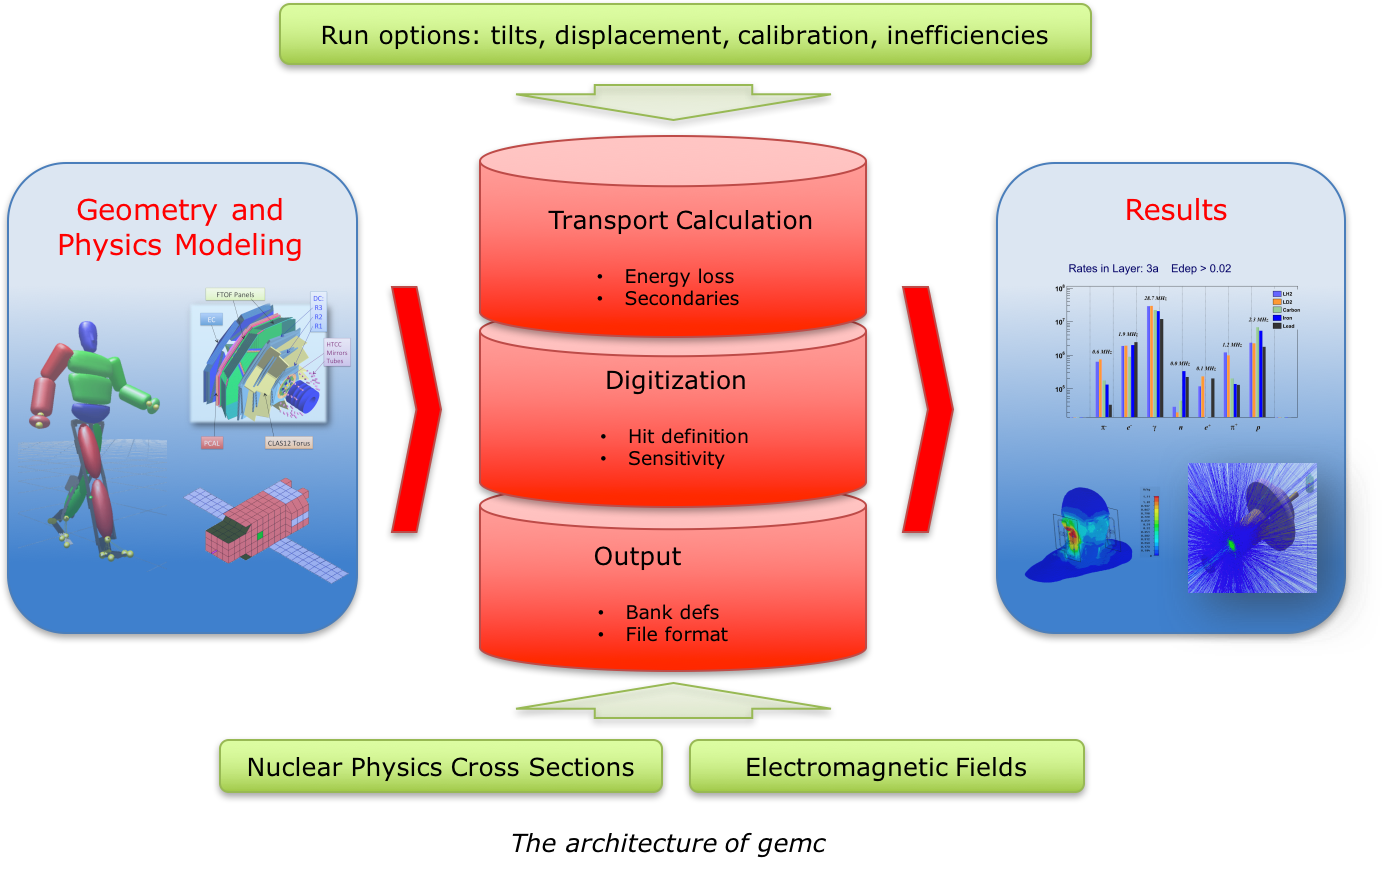
\includegraphics[width=0.65\textwidth]{Chapters/Ch3-Simulations/simulation_pipeline/pics/gemc_basics.png}
    \caption[GEMC Architecture]{GEMC architecture. Image from \parencite{Ungaro2020TheSimulation}.}
    \label{fig:gemc_architecture}
\end{figure}

Step (2) is straightforward after having been developed as discussed in \chref{Chapter:Experiment}. The distributions from \figref{fig:aao_norad_gen} after passing through the GEMC simulation, CLAS12 reconstruction software, and event selection are shown in \figref{fig:aao_norad_sim}, where the differences between the distributions is indicative of the acceptance cutoffs of the CLAS12 experiment. 


    \begin{figure}[H]
        \centering
        \subfloat[]{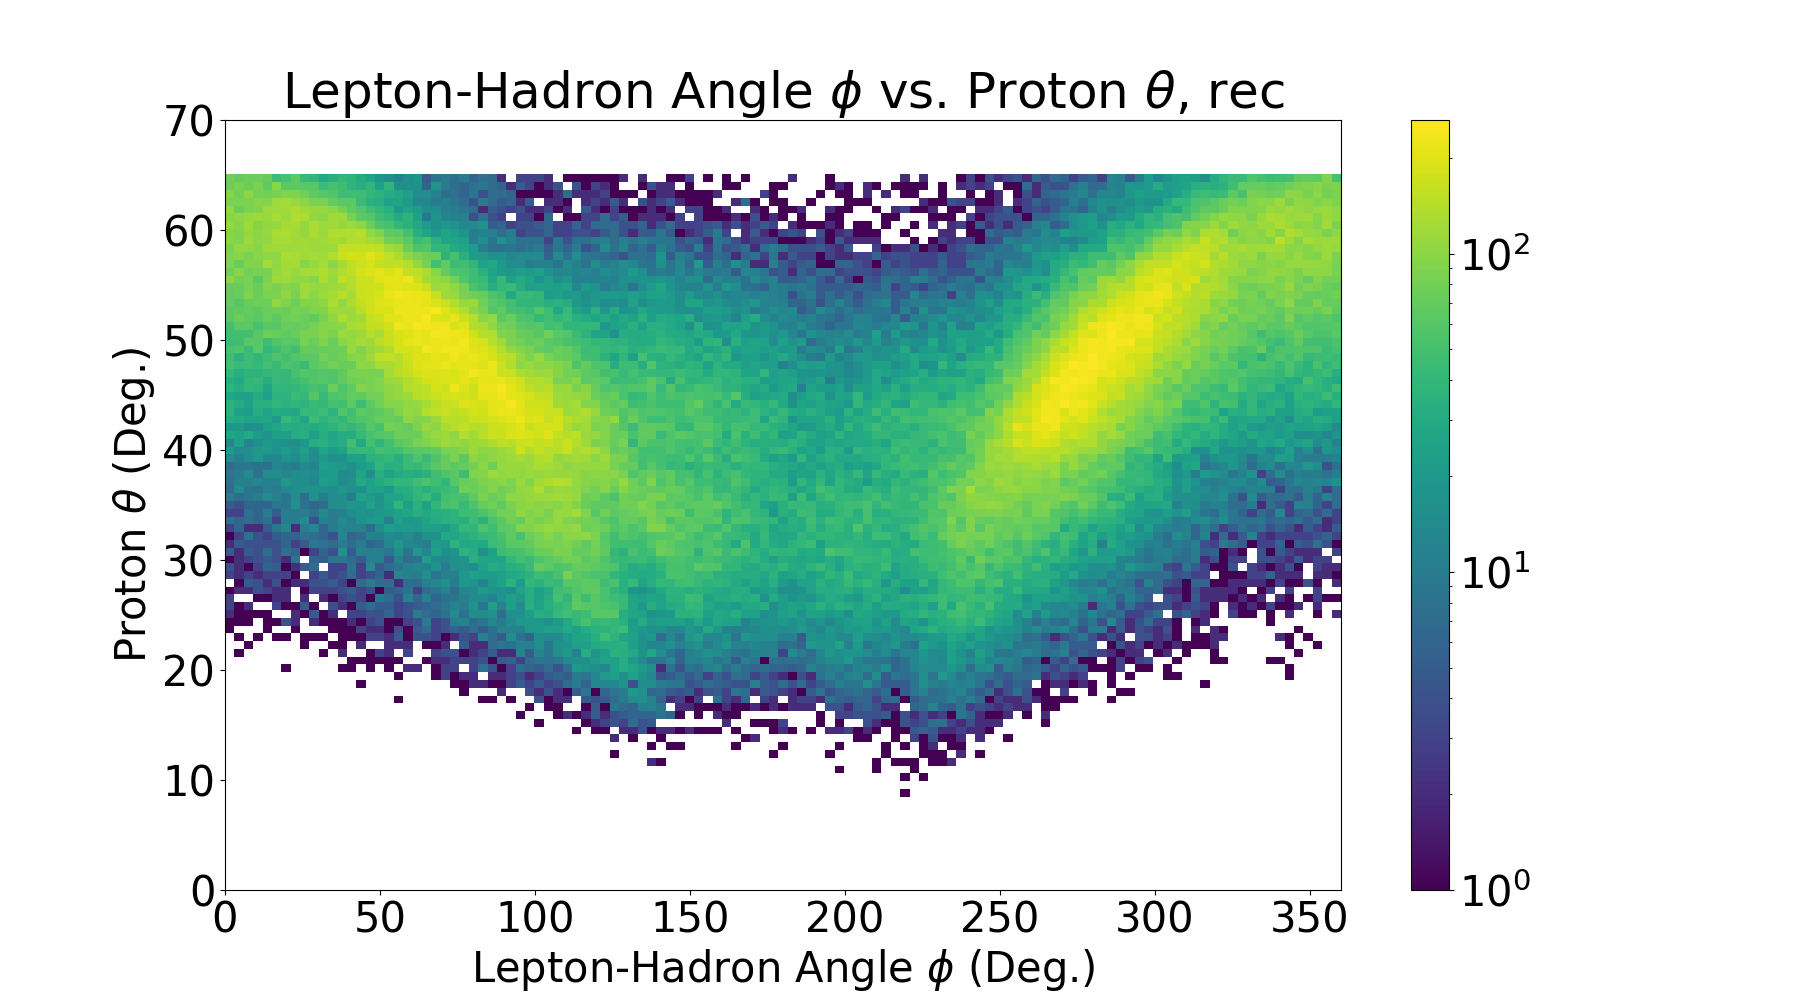
\includegraphics[width=0.5\textwidth]{Chapters/Ch3-Simulations/event_generation/pics/Lepton-Hadron_Angle_phi_vs_Proton_theta,_rec.png}}
        \hfill
        \subfloat[]{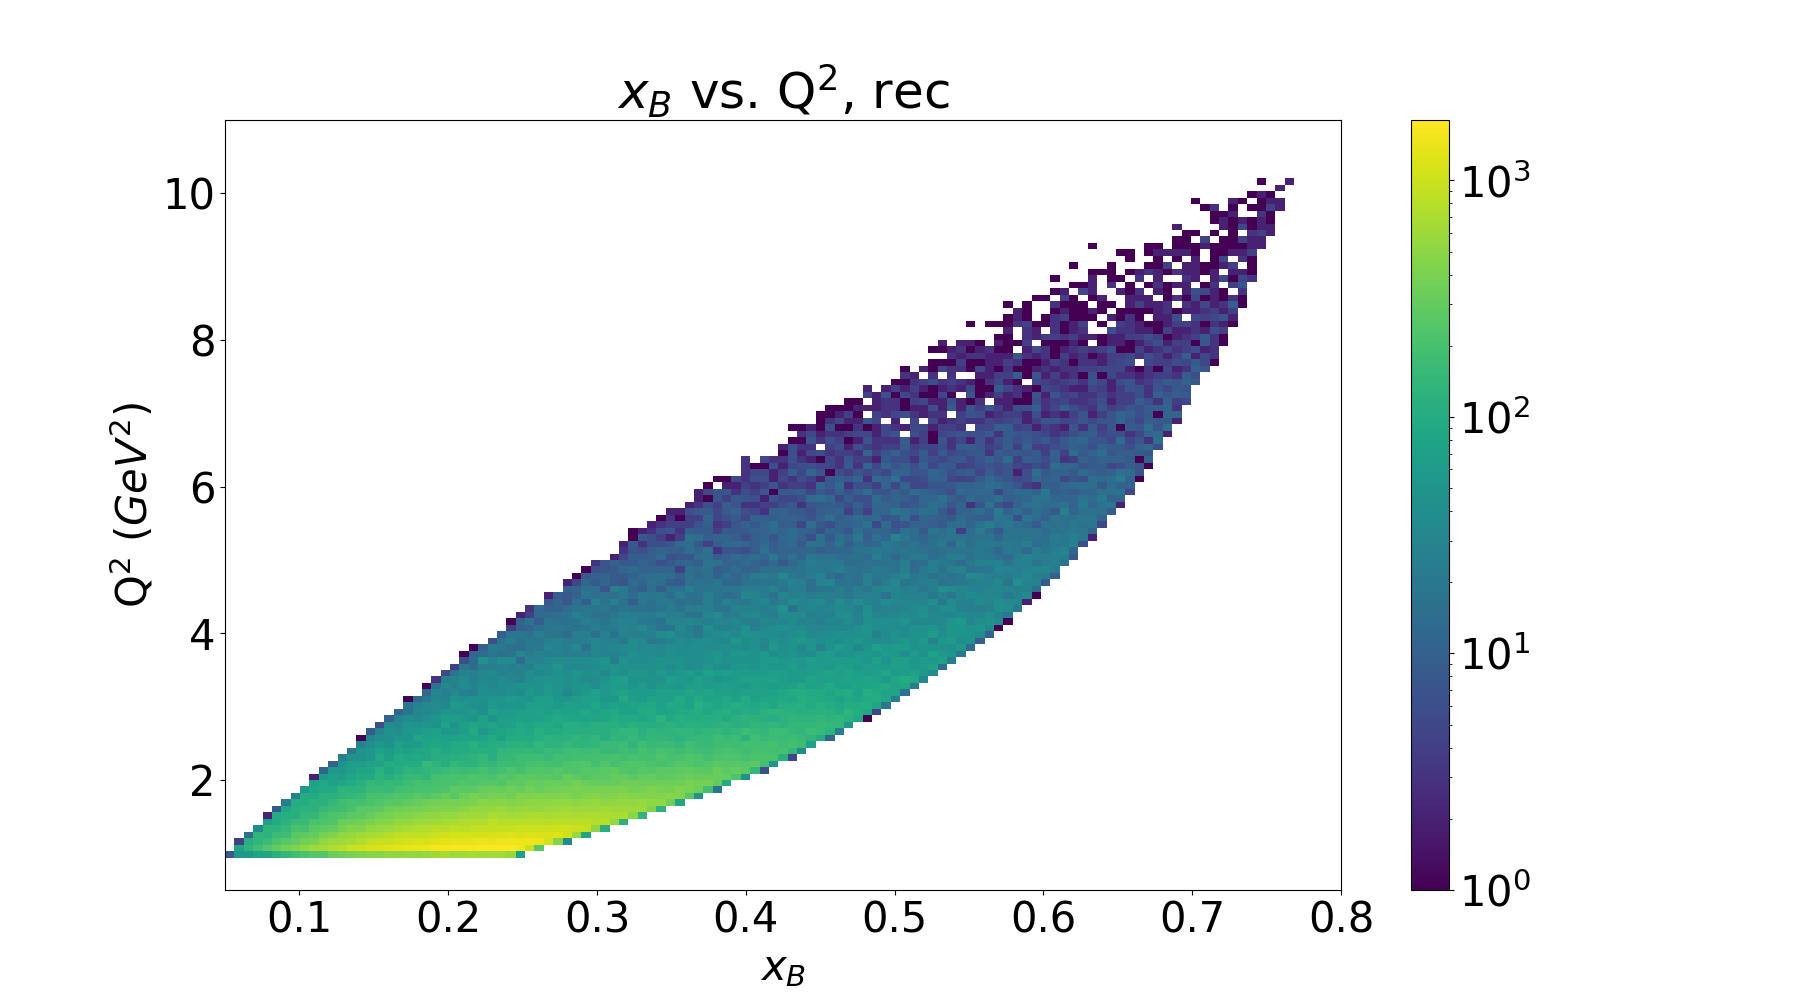
\includegraphics[width=0.5\textwidth]{Chapters/Ch3-Simulations/event_generation/pics/x_B_vs_Q2,_rec.png}}
        \caption[Reconstructed Event Distributions]{Reconstructed event distributions}\label{fig:aao_norad_sim}
    \end{figure}

\iffalse
    
    Event generation - fortran and c++ python wrapped
    geant4 docker gemc sysem
    reconstruction from part 2
    
    CLAASana
    
    this should talk about Geant4, GEMC, microphysics MCMC

\fi


    
        
